%%%%%%%%%%%%%%%%%%%%%%%%%%%%%%%%%%%%%%%%%
% Developer CV
% LaTeX Template
% Version 1.0 (28/1/19)
%
% This template originates from:
% http://www.LaTeXTemplates.com
%
% Authors:
% Jan Vorisek (jan@vorisek.me)
% Based on a template by Jan Küster (info@jankuester.com)
% Modified for LaTeX Templates by Vel (vel@LaTeXTemplates.com)
%
% License:
% The MIT License (see included LICENSE file)
%
%%%%%%%%%%%%%%%%%%%%%%%%%%%%%%%%%%%%%%%%%

%----------------------------------------------------------------------------------------
%	PACKAGES AND OTHER DOCUMENT CONFIGURATIONS
%----------------------------------------------------------------------------------------

\documentclass[9pt]{developercv} % Default font size, values from 8-12pt are recommended


%----------------------------------------------------------------------------------------

\begin{document}

%----------------------------------------------------------------------------------------
%	TITLE AND CONTACT INFORMATION
%----------------------------------------------------------------------------------------

\begin{minipage}[t]{0.45\textwidth} % 45% of the page width for name
	\vspace{-\baselineskip} % Required for vertically aligning minipages
	
	% If your name is very short, use just one of the lines below
	% If your name is very long, reduce the font size or make the minipage wider and reduce the others proportionately
	\colorbox{black}{{\huge\textcolor{white}{\textbf{\MakeUppercase{Jonas}}}}} % First name
	
	\colorbox{black}{{\huge\textcolor{white}{\textbf{\MakeUppercase{Schultheiss}}}}} % Last name
	
	\vspace{6pt}
	
	{\huge Full stack developer} % Career or current job title
\end{minipage}
\begin{minipage}[t]{0.32\textwidth} % 27.5% of the page width for the first row of icons
	\vspace{-\baselineskip} % Required for vertically aligning minipages
	
	% The first parameter is the FontAwesome icon name, the second is the box size and the third is the text
	% Other icons can be found by referring to fontawesome.pdf (supplied with the template) and using the word after \fa in the command for the icon you want
	\icon{MapMarker}{12}{Ettingen, Schweiz}\\
	\icon{Phone}{12}{+41 76 747 61 55}\\
	\icon{At}{12}{\href{mailto:contact@jonasschultheiss.dev}{contact@jonasschultheiss.dev}}\\	
\end{minipage}
\begin{figure}[!ht]
  \centering
  \colorbox{black}{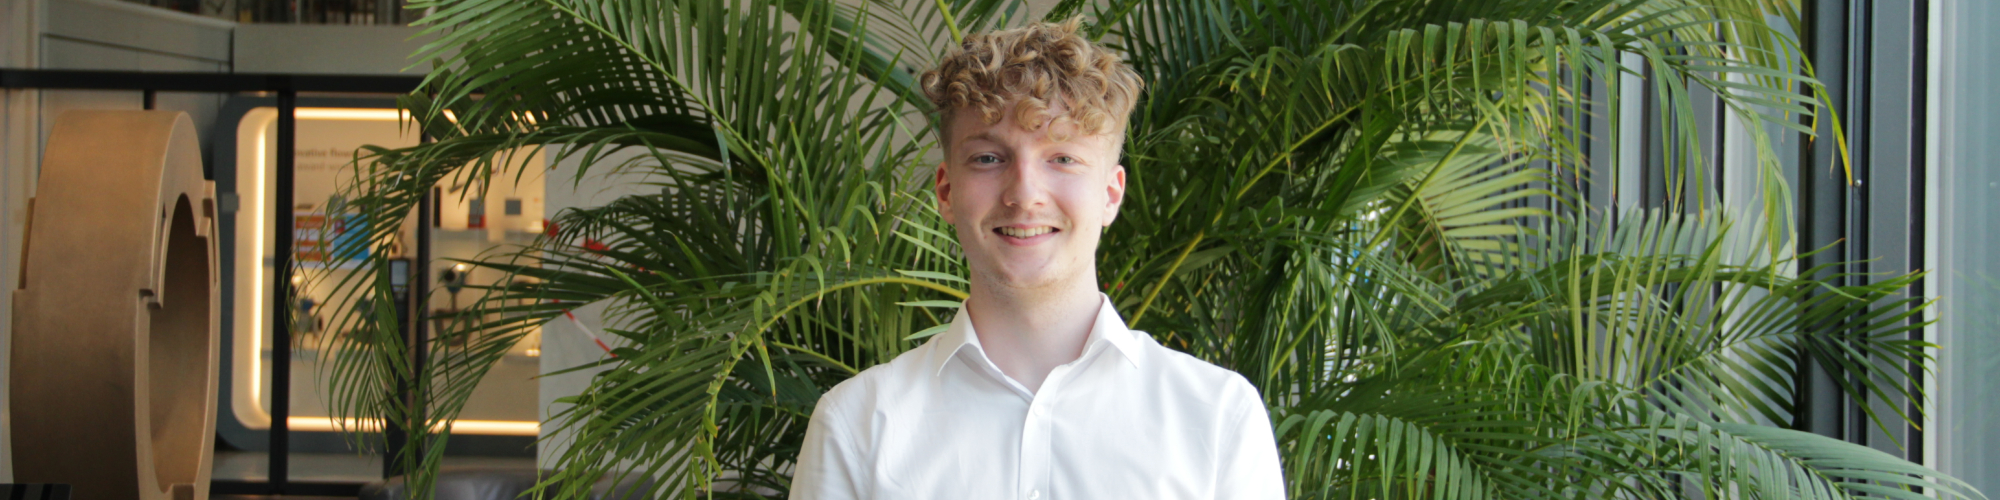
\includegraphics[width=1\linewidth]{./me.jpg}}
\end{figure}
\begin{minipage}[t]{0.23\textwidth} % 27.5% of the page width for the second row of icons
	\vspace{-\baselineskip} % Required for vertically aligning minipages
	
	% The first parameter is the FontAwesome icon name, the second is the box size and the third is the text
	% Other icons can be found by referring to fontawesome.pdf (supplied with the template) and using the word after \fa in the command for the icon you want
	\icon{Globe}{12}{\href{https://jonasschultheiss.dev}{jonasschultheiss.dev}}\\
	\icon{Github}{12}{\href{https://github.com/jonasschultheiss}{jonasschultheiss}}\\
	\icon{Twitter}{12}{\href{https://twitter.com/@SchultheissJ}{@SchultheissJ}}\\
\end{minipage}

\vspace{0.5cm}

%----------------------------------------------------------------------------------------
%	INTRODUCTION, SKILLS AND TECHNOLOGIES
%----------------------------------------------------------------------------------------

\cvsect{Zusammenfassung}

\begin{minipage}[t]{0.48\textwidth} % 40% of the page width for the introduction text
	\vspace{-\baselineskip} % Required for vertically aligning minipages
	
  Ich bin ein Informatiker EFZ aus der Schweiz, der derzeit bis Ende Juli 2021 als Auszubildender bei Endress+Hauser beschäftigt ist. Endress+Hauser ist der Marktführer für Messgeräte, die in der Industrie eingesetzt werden. Zum Portfolio gehören auch die IIoT-Plattform "Netilion", das Angebot von Komplettlösungen und verschiedene Dienstleistungen. Während der gesamten Lehre habe ich immer gezeigt, dass ich bereit bin mehr zu leisten, als von mir erwartet wurde, sowohl in Bezug auf die Arbeit in der Berufsschule als auch auf die Aufgaben im Betrieb.
\end{minipage}
\hfill % Whitespace between
\begin{minipage}[t]{0.48\textwidth} % 50% of the page for the skills bar chart
	\vspace{-\baselineskip} % Required for vertically aligning minipages
  Diese Grundlage hat mir ein solides technisches Skillset und arbeitsbasierte Erfahrung als Vorbereitung für eine Karriere in der Informatik gegeben.

Mein derzeitiger Stack besteht aus Next.js und Nest.js, aber das kann von Projekt zu Projekt variieren.

Ich bin daran interessiert, als Full-Stack-Entwickler in einem fortschrittlichen Unternehmen zu arbeiten, das Wert auf Teamarbeit, Kommunikation und moderne Technologien legt. Es ist mir wichtig, dass mir die Möglichkeit geboten wird, mich aktiv weiterzubilden, damit ich in der Webentwicklung auf dem neuesten Stand bleibe.
\end{minipage}

% \begin{center}
% 	\bubbles{5/Eclipse, 6/git, 4/Office, 3/Inkscape, 3/Blender}
% \end{center}

%----------------------------------------------------------------------------------------
%	EXPERIENCE
%----------------------------------------------------------------------------------------

\cvsect{BERUFSERFAHRUNG}

\begin{entrylist}
	\entry
		{08.2017 -- 07.2021}
		{Lehre als Informatiker EFZ, Fachr. Applikationsentwicklung}
		{\href{https://endress.com}{Endress+Hauser Process Solutions AG}}
		{Im Sommer 2017 habe ich bei Endress+Hauser meine Ausbildung zum Informatiker EFZ mit der Fachrichtung Anwendungsentwicklung begonnen. Im Schweizer Lehrlingssystem hat man pro Woche ein bis zwei Tage Berufsschule. Den Rest verbringt man im Betrieb. Im ersten Lehrjahr wurden die Grundlagen der Informatik vermittelt. Im Betrieb wurde ich von meinem Vorgesetzten intensiv in C\# unterrichtet.

    Im zweiten Lehrjahr habe ich mich auf JavaScript konzentriert. Ich bekam von meinem Arbeitgeber die Aufgabe, die vorhandenen Bash Skripte durch eine Node.js Applikation zu ersetzen. Diese werden in der Produktion eines Gerätes bzw. dessen Software eingesetzt. Die Bash Skripte waren alt, schwer zu warten und langsam. Dieses Projekt ermöglichte es mir, eine solide Grundlage in JavaScript und Node.js aufzubauen und das System für das Team benutzerfreundlicher zu machen.
    
    Ab dem dritten Lehrjahr beschäftigte ich mich intensiv mit der Webentwicklung. Ich verwendete React und erstellte von Grund auf diverse Websites, die im Training und/oder Sales eingesetzt werden, um das IIoT Angebot von Endress+Hauser für Kunden attraktiv und verständlicher zu machen. Außerdem arbeitete ich mehrere Monate lang mit dem Web-Entwicklungsteam zusammen. Während dieser Zeit habe ich eine Website erstellt, auf der der Kunde mit einem 3D Modell interagieren kann. Sie können mehr darüber auf meiner Portfolio Seite finden.\\ \texttt{Next.js}\slashsep\texttt{Nest.js}\slashsep\texttt{C\#}}
\end{entrylist}
%----------------------------------------------------------------------------------------
%	EDUCATION
%----------------------------------------------------------------------------------------

\cvsect{BILDUNG}

\begin{entrylist}
	\entry
		{08.2017 -- 07.2021}
		{Lehre als Informatiker EFZ, Fachr. Applikationsentwicklung}
		{\href{https://www.bbzbl.ch/}{BBZ-BL}}
		{Während meiner Ausbildung besuchte ich die BBZ-BL. Hier erhielt ich meine Grundausbildung in der Informatik. Verschiedene Schulprojekte sind auf meiner Website zu finden.}
	\entry
		{06.2012 -- 08.2017}
		{Sekundarschule, Niveau E}
		{\href{https://www.sektherwil.ch/}{Sekundarschule Therwil}}
		{}
\end{entrylist}
\pagebreak

%----------------------------------------------------------------------------------------
%	Additional experiences
%----------------------------------------------------------------------------------------

\cvsect{ZUSÄTZLICHE ERFAHRUNGEN}

\begin{entrylist}
	\entry
		{10.2020}
		{E+H PCPS Fedex Day 2020}
		{\href{https://endress.com}{Endress+Hauser Process Solutions AG}}
		{Dies war der dritte Hackathon, an dem ich teilgenommen habe. Wir nutzten eine embedded Komponente um Stehlampen anzusteuern. Dafür erstellten wir ein eigenes Script, ein Node.js Backend und ein React Frontend. Schlussendlich konnten wir die Lampe ein-/ausschalten, die Helligkeit regulieren und die Wärme in Kelvin einstellen. Der Plan war, daraus ein komplettes internes Projekt zu machen, bei dem ein Mitarbeiter ein eigenes Profil erstellen kann. Allerdings ist derzeit unklar, ob das Unternehmen daraus ein vollständiges Projekt machen wird.\\ \texttt{React}\slashsep\texttt{Node.js}}
	\entry
		{12.09.2020}
		{ICTskills2020: Die Schweizermeisterschaften im ICT-Berufsfeld}
		{\href{https://www.ict-berufsbildung.ch/}{ICT-Berufsbildung Schweiz}}
		{Die ICTSkills sind die Schweizer Berufsmeisterschaften in der IT Branche. Nachdem ich mich in regionalen Runden erfolgreich qualifiziert hatte, nahm ich am nationalen Wettbewerb in Bern teil.
    An einem Tag mussten wir verschiedene Aufgaben in HTML, CSS, JavaScript, ReGeX, PHP und MySQL lösen.  Das ist mir ganz gut gelungen. Leider musste ich fast alle PHP Punkte abgeben, da ich mich während der Ausbildung nicht auf PHP, sondern auf Node.js konzentriert habe.
    Trotzdem konnte ich durch die Vorbereitung und die Berufsmeisterschaft selbst viel lernen und bereits gelerntes nochmals vertiefen.\\ \texttt{HTML5}\slashsep\texttt{CSS3}\slashsep\texttt{JavaScript}\slashsep\texttt{ReGeX}\slashsep\texttt{PHP}\slashsep\texttt{SQL}}
	\entry
		{10.2019 -- 11.2019}
		{C++ Workshop}
		{\href{https://ethz.ch/}{ETH Zürich}}
		{Dieser zweiwöchige C++ Workshop wurde von Studenten der ETH Zürich geleitet. Es mussten verschiedene Aufgaben gelöst werden, bei denen die Laufzeit und die Grösse des Arbeitsspeichers berücksichtigt werden mussten. Die Studenten erklärten in Theorieblöcken mehr über C++, die Big O Notation und andere Konzepte. Dabei konnte ich sehr viel lernen und mein Wissen in C++ vertiefen.\\ \texttt{C++}}
	\entry
		{10.2019}
		{E+H PCPS Fedex Day 2019}
		{\href{https://endress.com}{Endress+Hauser Process Solutions AG}}
		{Der zweite Hackathon, an dem ich teilgenommen habe. Wir haben den Prototyp vom letztjährigen Hackathon verbessert. Wir haben ihn wieder von Grund auf neu gebaut, aber unsere Erfahrungen aus dem Vorjahr genutzt. Der größte Unterschied zum letzten Jahr war, dass wir das express.js Backend durch die Firebase Realtime Database von Google ersetzt haben. Dies ermöglichte uns, einen Wert direkt zu aktualisieren oder auf eine Änderung zu reagieren, ohne dass wir die Struktur dafür aufbauen mussten.\\ \texttt{React}\slashsep\texttt{Firebase}}
	\entry
		{10.2018}
		{E+H PCPS Fedex Day 2018}
		{\href{https://endress.com}{Endress+Hauser Process Solutions AG}}
		{Der erste Hackathon, an dem ich teilgenommen habe. Wir haben einen Prototyp für ein IoT-System erstellt, das die Luftqualität in Besprechungsräumen misst und auf einer Website anzeigt.\\ \texttt{Node.js}\slashsep\texttt{MongoDB}}
	\entry
		{09.2018 -- 11.2018}
		{AppQuest}
		{\href{https://appquest.ch/}{Hochschule für Technik Rapperswil and Berner Fachhochschule}}
		{Kurs zur mobilen Entwicklung mit swift. Wir bekamen verschiedene Herausforderungen. Um diese Herausforderungen zu meistern, musste man verschiedene kleine Apps programmieren. Ein Beispiel wäre eine App, die einen Rotfilter über die Ausgabe der Kamera legte, sodass man versteckte Botschaften in einem Bild lesen konnte.

    Wir haben diese Apps gemacht, weil sie für eine Schatzsuche benötigt wurden. Dort bekamen wir Hinweise, die man nur lesen konnte, wenn man seine App richtig programmierte.\\ \texttt{Swift}\slashsep\texttt{iOS}}
\end{entrylist}

%----------------------------------------------------------------------------------------
%	ADDITIONAL INFORMATION
%----------------------------------------------------------------------------------------

\begin{minipage}[t]{0.3\textwidth}
	\vspace{-\baselineskip} % Required for vertically aligning minipages

	\cvsect{Sprachen}
	
	\textbf{Deutsch} - Muttersprache\\
	\textbf{Englisch} - Fachliche Eignung\\
\end{minipage}
\hfill
\begin{minipage}[t]{0.3\textwidth}
	\vspace{-\baselineskip} % Required for vertically aligning minipages
	
	\cvsect{Hobbies}
	
	In meiner Freizeit spiele ich gerne mit meinen Kollegen Fussball, Volleyball oder Basketball. Ausserdem habe ich noch einen kleinen Bruder, mit dem ich auch gerne meine Freizeit verbringe.
\end{minipage}
\hfill
\begin{minipage}[t]{0.3\textwidth}
	\vspace{-\baselineskip} % Required for vertically aligning minipages
	
	\cvsect{Non profit}
	
  Ich habe zusammen mit Freunden und Bekannten den Verein "PR1SM" gegründet, welcher sich aktiv mit digitalen Medien und regionalem E-Sports beschäftigt.
\end{minipage}

%----------------------------------------------------------------------------------------

\end{document}
